
\documentclass[conference]{IEEEtran}
\ifCLASSINFOpdf
  \usepackage[pdftex]{graphicx}
\hyphenation{op-tical net-works semi-conduc-tor}


\begin{document}
\title{Decision Tree Classifiers with GA based feature selectors}


% author names and affiliations
% use a multiple column layout for up to three different
% affiliations
\author{
\IEEEauthorblockN{Samir Sheriff}
\IEEEauthorblockA{BE 7 semester\\ Department of Computer Science\\RV College of Engineering\\
Email:samiriff@gmail.com}
\and
\IEEEauthorblockN{Satvik N}
\IEEEauthorblockA{BE 7 semester\\ Department of Computer Science\\RV College of Engineering\\
Email:nsatvik@gmail.com}
\and
\IEEEauthorblockN{Mrs. Shanta Rangaswamy }
\IEEEauthorblockA{Assistant Professor\\ Department of Computer Science\\RV College of Engineering\\
Email:shantharangaswamy@rvce.edu.in}
}




% make the title area
\maketitle


\begin{abstract}
%\boldmath
Machine Learning techniques like decision trees can learn classification patterns  from training data and generate classifiers that then are used to solve decision problems. In general, the input data to classifiers is a set of features, but not all of features are relevant
to the classes to be classified.Although the problem of finding an optimal decision tree has received attention, it is a hard  optimization problem.


 In this paper, we use a genetic algorithm to select a subset of input features for decision tree
classifiers, with a goal of increasing the efficiency of the decision tree and thus increasing it’s efficiency to solve the decision problem.
\end{abstract}
\begin{keywords}
decision tree, machine learning, genetic algorithms, decision problems.
\end{keywords}

\IEEEpeerreviewmaketitle



\section{Introduction}
Decision trees have been well studied and widely used in knowledge discovery and decision support systems. Classification with decision trees involves constructing trees where the leaves represent classifications and the branches represent feature-based splits that lead to the classifications. These trees approximate discrete-valued target functions as trees and are a widely used practical method for inductive inference. Decision trees have prospered in knowledge discovery and decision support systems because of their natural and intuitive paradigm to classify a pattern through a sequence of questions. 


 A key problem is how to choose the features (attributes) of the input training data on which
learning will take place. Since not every feature of the training  data may be relevant to the classification task and, in the worse case, irrelevant features may introduce noise and redundancy into the design of classifiers, choosing a good subset of features will be critical to improve the performance of classifiers. 



In this paper we use a genetic algorithm to find an optimal subset of features for decision tree classifiers based on few generic data sets.


\section{Introduction to Decision Trees and Genetic Algorithms}
\subsection{Decision Trees}
The decision tree classifier is a machine learning technique for building classifiers. A decision tree is made of
decision(internal) nodes and leaf nodes. Each decision/internal node corresponds to
a test X over a single attribute of the input data and has a number
of branches, each of which handles an outcome of the test X. In binary decision trees there are only two branches from a decision/internal node.
Each leaf node represents a class that is the result of decision for
a case.



The process of constructing a decision tree is basically a divide and conquer process. A set T of training data consists of k
classes $( C_1, C_2,$…,$ C_k )$. If T only consists of cases of one single
class, T will be a leaf. If T contains
cases of mixed classes (i.e. more than one class), a test based on
some attribute $a_i$ of the training data will be carried and T will
be split into n subsets $( T_1 , T_2 , …, T_n)$, where n is the number of
outcomes of the test over attribute $a_i$ . The same process of
constructing decision tree is recursively performed over each $T_j$ ,
where $1\leq j \leq n$ , until every subset belongs to a single class.



The problem here is how to choose the best attribute for each
decision node during construction of the decision tree. The
criterion that C4.5 chooses is Gain Ratio Criterion. The basic idea
of this criterion is to, at each splitting step, choose an attribute
which provides the maximum information gain while reducing
the bias in favor of tests with many outcomes by normalization.



Once a decision tree is built, it can be used to classify testing data
that has the same features as the training data. Starting from the
root node of decision tree, the test is carried out on the same
attribute of the testing case as the root node represents. The
decision process takes the branch whose condition is satisfied by
the value of tested attribute. This branch leads the decision
process to a child of the root node. The same process is
recursively executed until a leaf node is reached. The leaf node is
associated with a class that is assigned to the test case.


\subsection{Genetic Algorithms}
Genetic Algorithms have been successfully applied to
solve search and optimization problems. The basic idea of a GA
is to search a hypothesis space to find the best hypothesis. A pool
of initial hypotheses called a population is randomly generated
and each hypothesis is evaluated with a fitness function.


Hypotheses with greater fitness have higher probability of being
chosen to create the next generation. Some fraction of the best
hypotheses may be retrained into the next generation, the rest
undergo genetic operations such as crossover and mutation to
generate new hypotheses. The size of a population is the same for
all generations in our implementation. This process is iterated
until either a predefined fitness criterion is met or the preset
maximum number of generations is reached.
\begin{figure}[h!]
  
  \centering
    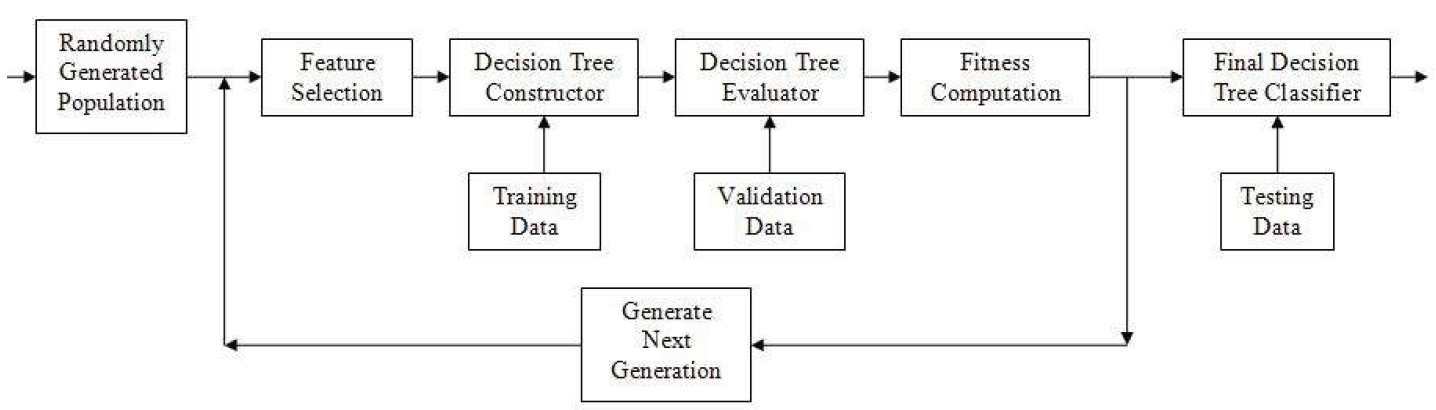
\includegraphics[scale=0.25]{dfd.png}
\caption{The data flow in DT/GA Hybrid Classifier.}
\end{figure}


A GA generally has four components. A population of
individuals where each individual in the population represents a
possible solution. A fitness function which is an evaluation
function by which we can tell if an individual is a good solution
or not. A selection function which decides how to pick good
individuals from the current population for creating the next
generation. Genetic operators such as crossover and mutation
which explore new regions of search space while keeping some of
the current information at the same time.
The following is a typical GA procedure:
\begin{verbatim}
Procedure GA
Begin
___Initialize population;
___Evaluate population members;
___While not an optimal solution do
___Begin
______Select parents from population;
______GA operation on parents;
______Evaluate offspring;
______Set offspring equal to population;
___End
End
\end{verbatim}
\subsection{GA-Based Feature Selection for Decision Trees}
In this algorithm, the search component is a GA and the
evaluation component is a decision tree. A detailed description of
this algorithm is shown in Figure 1. The initial population is
randomly generated. Every individual of the population has N
genes, each of which represents a feature of the input data and
can be assigned to 1 or 0. 1 means the represented feature is used
during constructing decision trees; 0 means it is not used. As a
result, each individual in the population represents a choice of
available features. For each individual in the current population, a
decision tree is built using the C4.5 program. This resulting
decision tree is then tested over validation data sets, which
generate classification error rates. The fitness of this
individual is the aggregate total of these classification error rates.
The lower the classification error rate, the better the fitness of the
individual.
Once the fitness values of all individuals of the current population
have been computed, the GA begins to generate next generation
as follows:
\begin{enumerate}
\item{}Choose individuals according to Rank Selection method.
\item{}Use two point crossover to exchange genes between parents to
create offspring.
\item{}Perform a bit level mutation to each offspring.
\item{}Keep two elite parents and replace all other individuals of
current population with offspring.
\end{enumerate}
The procedure above is iteratively executed until the maximum
number of generations is reached. Finally, the best
individual of the last generation is chosen to build the final
decision tree classifier, which is tested on the test data set.

\section{Implementation and Results}
The decision tree based classifier was implemented in Java. The implementation is generic so that it can be applied to any classification problem.


The DT/GA hybrid classifiers were tested with three classification problems. They are
\begin{itemize}
\item{Classifying Horse blood samples}
\item{Determining the portability of water}
\item{Determining the quality of the whine}
\end{itemize}

The results with the GA based optimization is shown in the Figure 2.
\begin{figure}[h!]
  
  \centering
    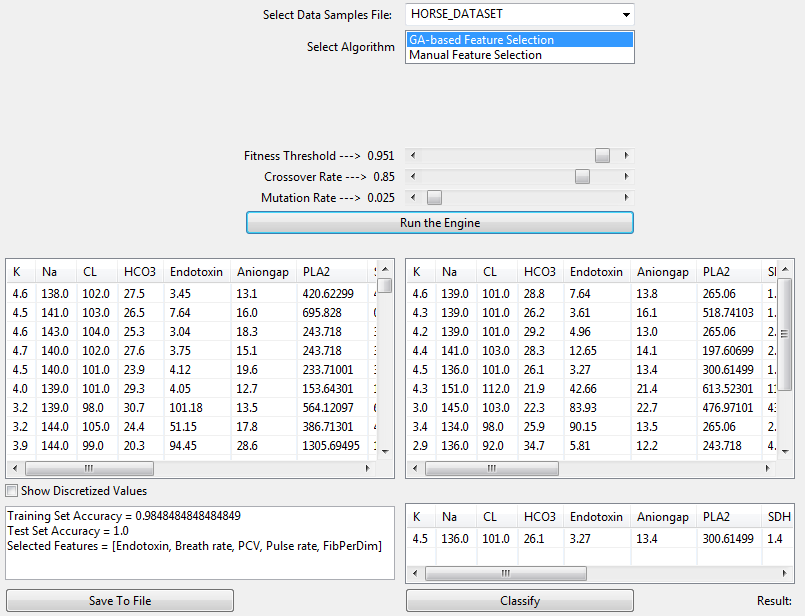
\includegraphics[scale=0.4]{ga_algo_stats.png}
\caption{DT built with GA based feature selector.}
\end{figure}

The results obtained with manual feature selection is shown in Figure 3.
\begin{figure}[h!]
  
  \centering
    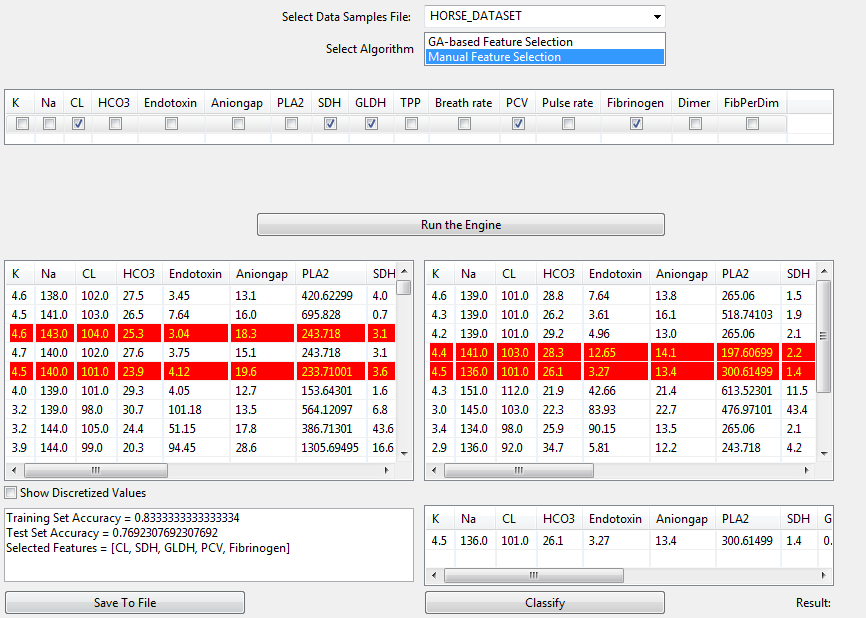
\includegraphics[scale=0.4]{manual_sel_stats.png}
\caption{DT built with manual feature selection.}
\end{figure}
\section{Conclusion}
The genetic algorithm and decision tree hybrid was able to
outperform the decision tree algorithm without feature selection.
We believe that this improvement is due to the fact that the
hybrid approach is able to focus on relevant features and
eliminate unnecessary or distracting features. This initial filtering
is able to improve the classification abilities of the decision tree.
The algorithm does take longer to execute than the standard
decision tree; however, its non-deterministic process is able to
make better decision trees. The training process needs only to be
done once. The classification process takes the same amount of
time for the hybrid and non-hybrid systems.

\section{Future Work}
The hybrid GA /decision tree algorithm needs to be tested more
in depth for its true potential. A forest of decision trees will be
constructed from the combination of four final decision trees,
each for one major attack category. The final decision will be
made through a voting algorithm. We will then compare the
overall classification ability of the hybrid algorithm with other
machine learning algorithms in the literature.


\begin{thebibliography}{1}

\bibitem{textbook}
Hua;Kien A., Wu;Annie S.; Chen;Bing, Stein;Gary
\emph{Decision Tree Classifier For Network Intrusion Detection
With GA-based Feature Selection}

\bibitem{paper}
Jing Xu, Ming Zhao,José Fortes, Robert Carpenter,
Mazin Yousif. \emph{Autonomic resource management in virtualized data centers using
fuzzy logic-based approaches} Cluster Comput (2008) 11: 213–227
DOI 10.1007/s10586-008-0060-0
\bibitem{paper}
T. Wood et al., \emph{Sandpiper.Black-box and gray-box resource management for virtual machines}, Computer Network (2009), doi:10.1016/j.comnet.2009.04.014
\end{thebibliography}

\end{document}


